% Move stuff about ENSO events to results?

% Some of the claims in the concluding paragraph of SSTA may be
% slightly grandiose

% Check reasoning behind NDVI spatial response discrepancy explanation
\section{Discussion}
\label{sec:disc}
\subsection{Thresholding}
\label{sec:disc:thresh}
In Section \ref{sec:method:thr} we described our method for
thresholding images, namely using Otsu's method. Figure \ref{fig:allp}
is illustrative of the efficacy of this method, applying it to all
land pixels for a single day (1/6/2008). Figure \ref{fig:allp_raw}
shows the raw image from EUMETSAT, where cloud is clearly visible over
western and equatorial Africa. Figure \ref{fig:allp_hist} shows the
distribution of land pixels in Figure \ref{fig:allp_raw}. It is not
clear whether the distribution is bimodal or log-normal, though it
could be said that there are two peaks: one at a pixel value of $\sim50$
and the other at a pixel value of $\sim110$. The broadness of this
distribution is caused by taking values from the entire image, whereas
in fact some places on the planet will be brighter in VIS0.8 than
others. We have then applied an Otsu threshold to categorise pixels as
`land' or `cloud', shown as white and green on the histogram. This is
a crude way of doing things, and is only done to illustrate the
process -- in reality, the Otsu threshold is calculated for \emph{each}
pixel from the distribution of its values over a period of time, so
the threshold value is more accurately scaled to that pixel. Figure
\ref{fig:allp_im} shows the land pixels from Figure \ref{fig:allp_raw}
where each pixels colour has been assigned according to whether it was
categorised as `land', `cloud' or masked out. Using this very simple
threshold manages to catch most of the cloud in western and equatorial
Africa, although it clearly fails miserably over the Sahara. In our
analysis we have overcome the shortcomings of the thresholding in the
desert by avoiding arid regions.
\begin{figure*}
  \centering
  \subcaptionbox{Raw image from
    EUMETSAT.\label{fig:allp_raw}}
                [0.3\textwidth]
                {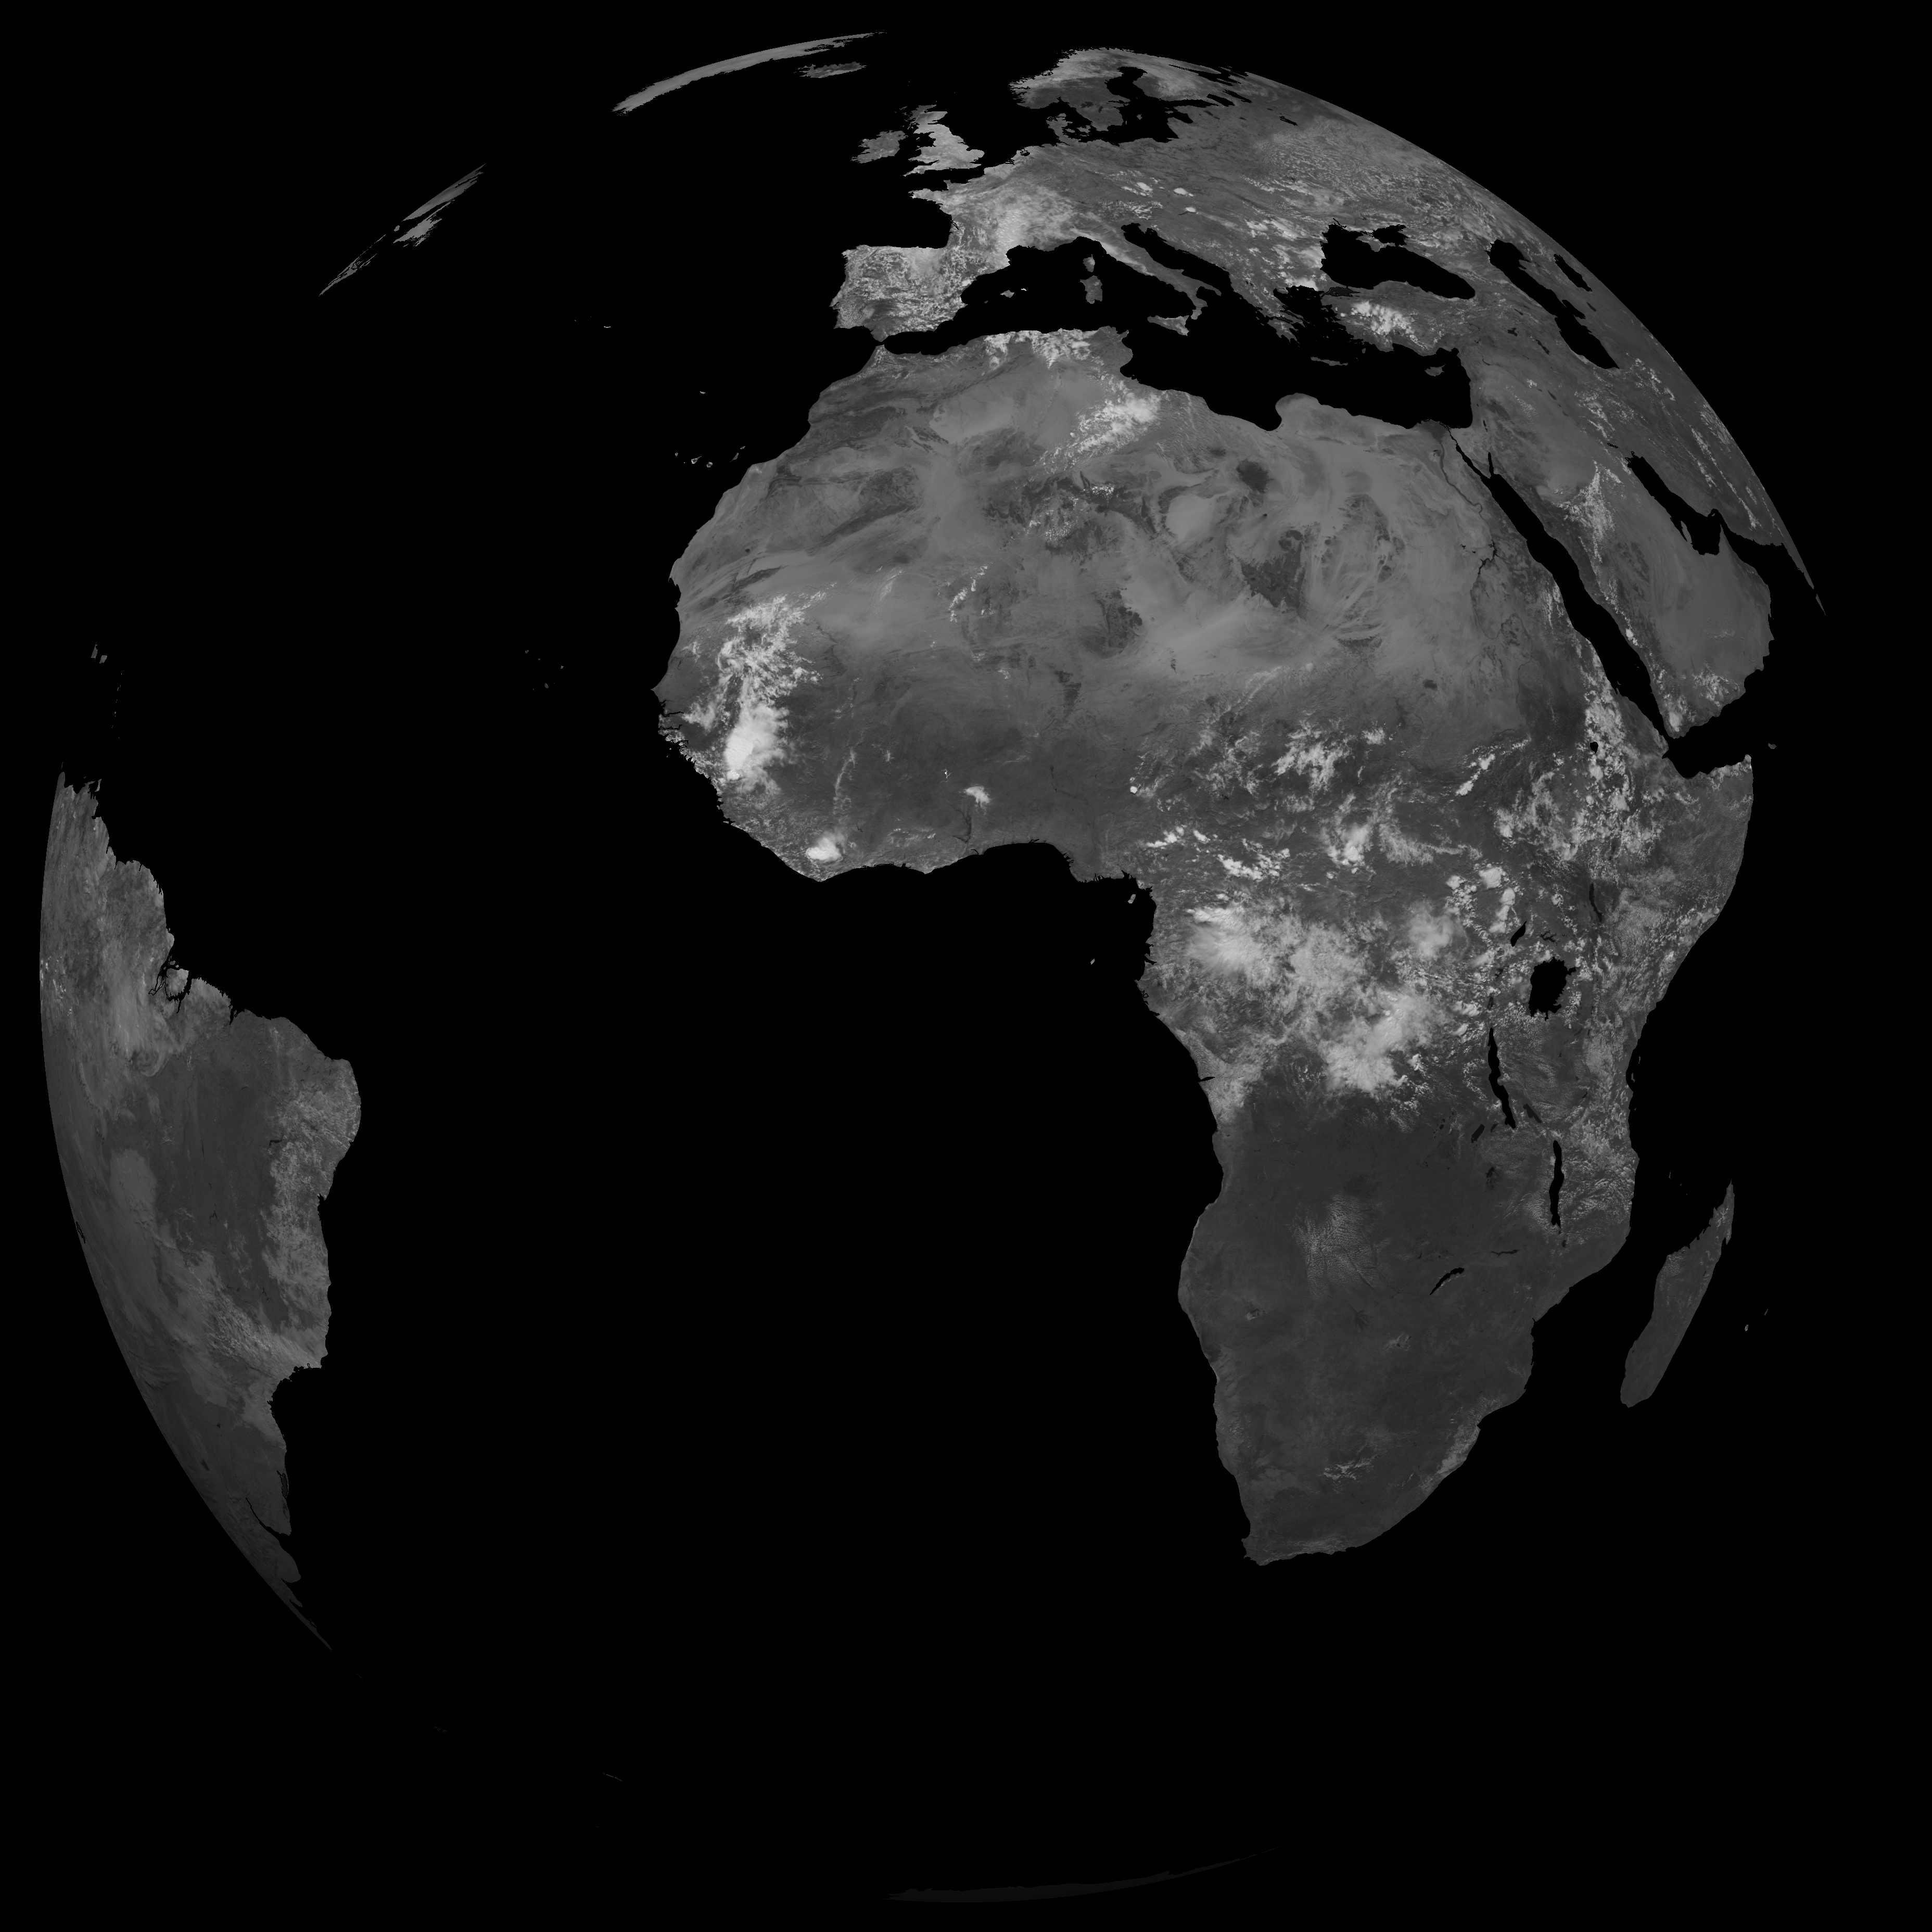
\includegraphics[width=0.3\textwidth]{figures/raw_im_all_pixels_01_06_2008_vis8}}
  ~
  \subcaptionbox{Histogram of the distribution of all the
    land pixels in Figure \ref{fig:allp_raw}. Green
    indicates where a pixel has been classified as `land'
    and white indicates `cloud' and black corresponds to
    masked pixels.\label{fig:allp_hist}}
                [0.33\textwidth]
                {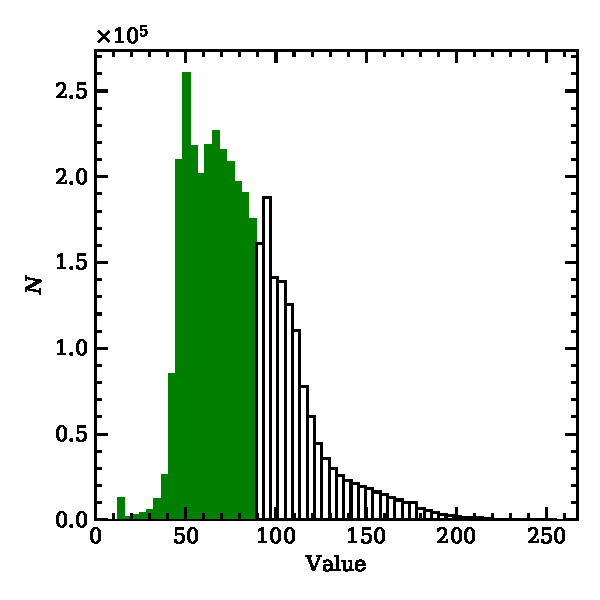
\includegraphics[width=0.33\textwidth]{figures/hist_all_pixels_01_06_2008_vis8}}
  ~
  \subcaptionbox{The image in Figure
    \ref{fig:allp_raw} masked and
    thresholded, so that the colour of each
    pixel corresponds to its classification
    as `land', `cloud' or masked
    out.\label{fig:allp_im}}
                [0.3\textwidth]
                {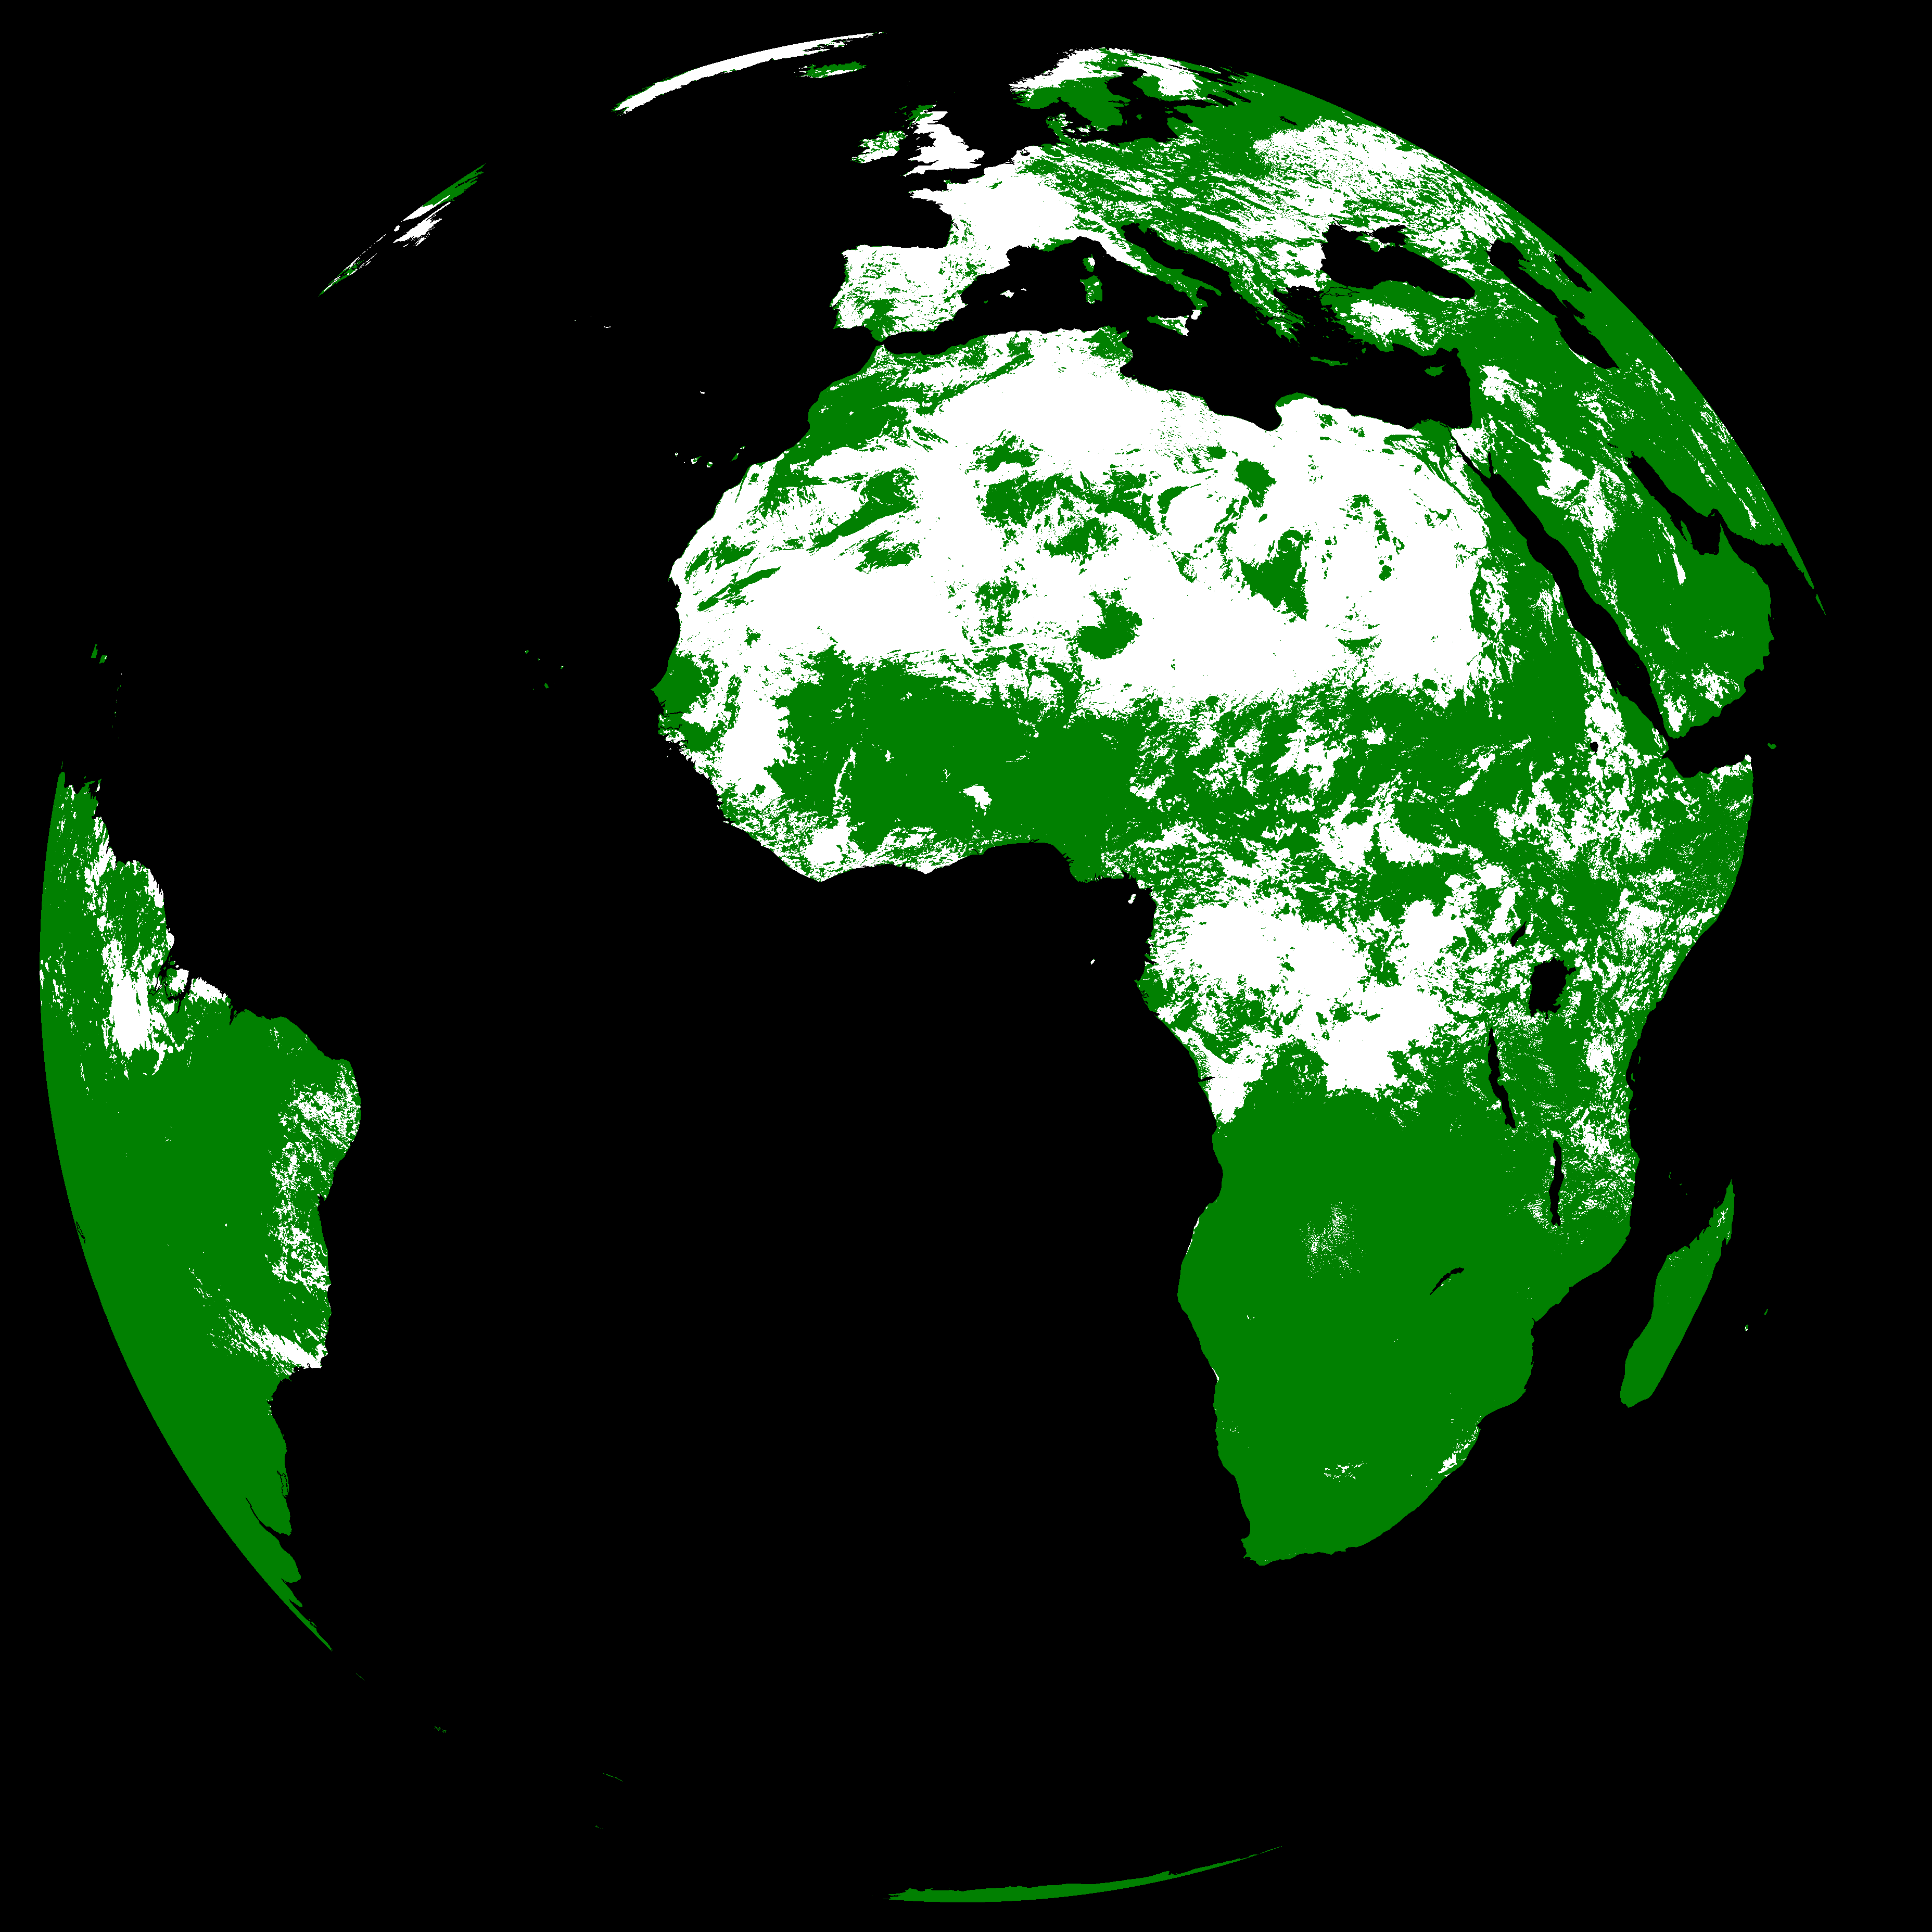
\includegraphics[width=0.3\textwidth]{figures/im_all_pixels_01_06_2008_vis8}}
  \caption{Thresholding of the image for 1/6/2008 in the VIS0.8 band.}
  \label{fig:allp}
\end{figure*}
It is useful to explore thresholding on the entire distribution, but
more relevant to our analysis is to see how it works for single
pixels. Figures \ref{pix_d_south} and \ref{pix_d_east} show the
normalised pixel distributions for South Africa and East Africa, for
three different pixels in the VIS0.6 and VIS0.8 bands. Also shown on
the plot are various statistics of the data, including the value of
the threshold calculated with Otsu's method, the mean of the entire
dataset, the median of the entire dataset, the mean of the data less
than the Otsu threshold and a Gaussian fit of the data less than the
Otsu threshold. It can be seen from the figures, that the fitted
Gaussian agrees fairly well with the data below the Otsu
threshold. This indicates that our method for producing cloud masks is
applicable -- we say that a pixel is classified as clear if it has a
value less than the value of the `ground' pixel plus some
uncertainty. The normal distribution of the values around the `ground'
value is as we expect, because some days the pixel will be in shade
and some days there will be some wispy cloud that we are unable to
detect. Here, the value of the `ground' pixel is the mean and the
uncertainty is the standard deviation of data below the threshold. It
is also interesting to note that the median returns a similar value to
the mean of the data below the threshold, although it does tend to
slightly overestimate.
\begin{figure*}
  \centering
  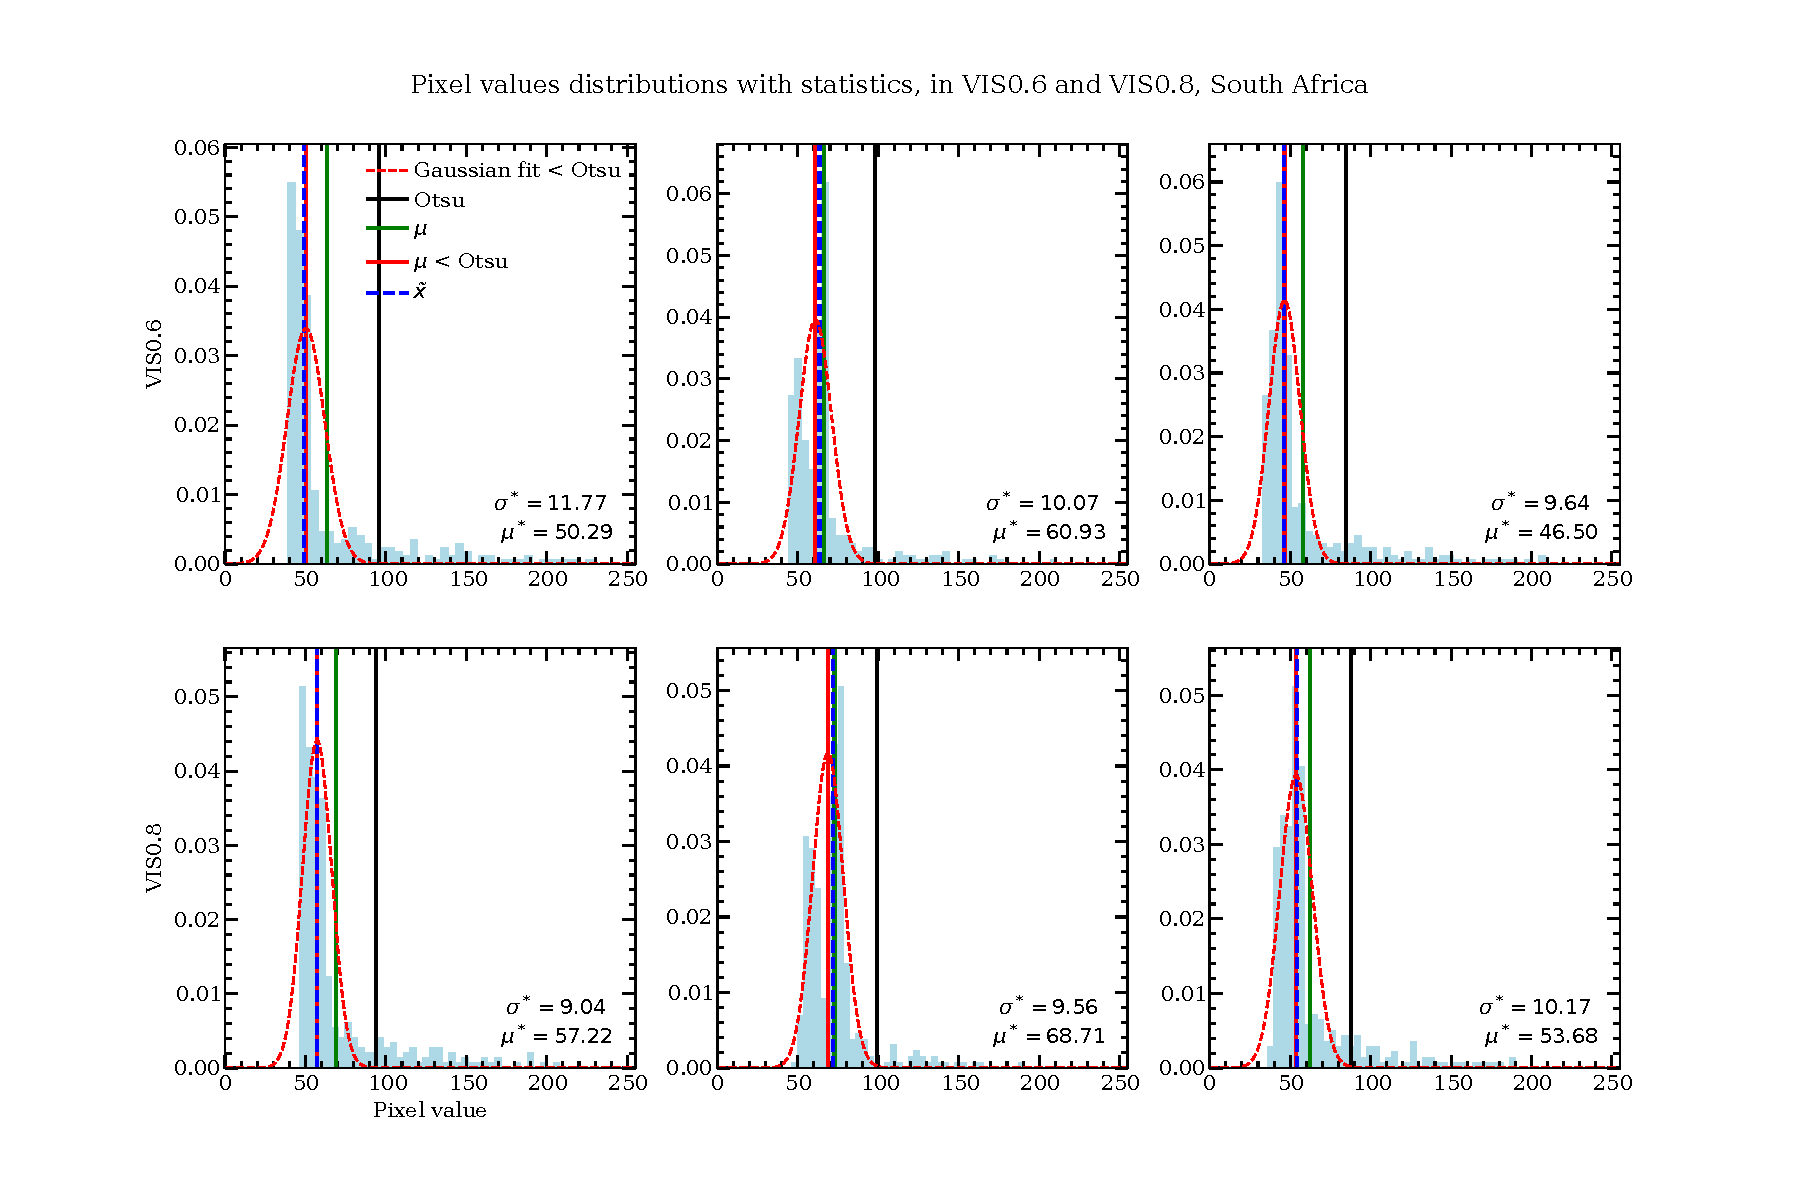
\includegraphics[width=\textwidth]{figures/pixel_distributions_stats_capetown}
  \caption{Normalised pixel distributions South Africa in the VIS0.8
    and VIS0.6 bands, for three pixels. Shown are the Otsu threshold
    (black), the mean of the entire dataset (green), the median of the
    entire dataset (dashed blue), the mean of the values below the
    Otsu threshold (red) and a Gaussian fit to the data below the Otsu
    threshold (dashed red). In the bottom right are the values for the
    mean $\mu$ and standard deviation $\sigma$ of the fitted Gaussian. The
    key point to note is how well the Gaussian fits the data below the
    threshold. This indicates that our method of using the mean of the
    values below the Otsu threshold to calculate a cloud free image
    (with the standard deviation as the uncertainty) is sound. Also
    interesting to note is how close the median is to this mean value,
    although it is usually an overestimate.}
  \label{fig:pix_d_south}
\end{figure*}

\begin{figure*}
  \centering
  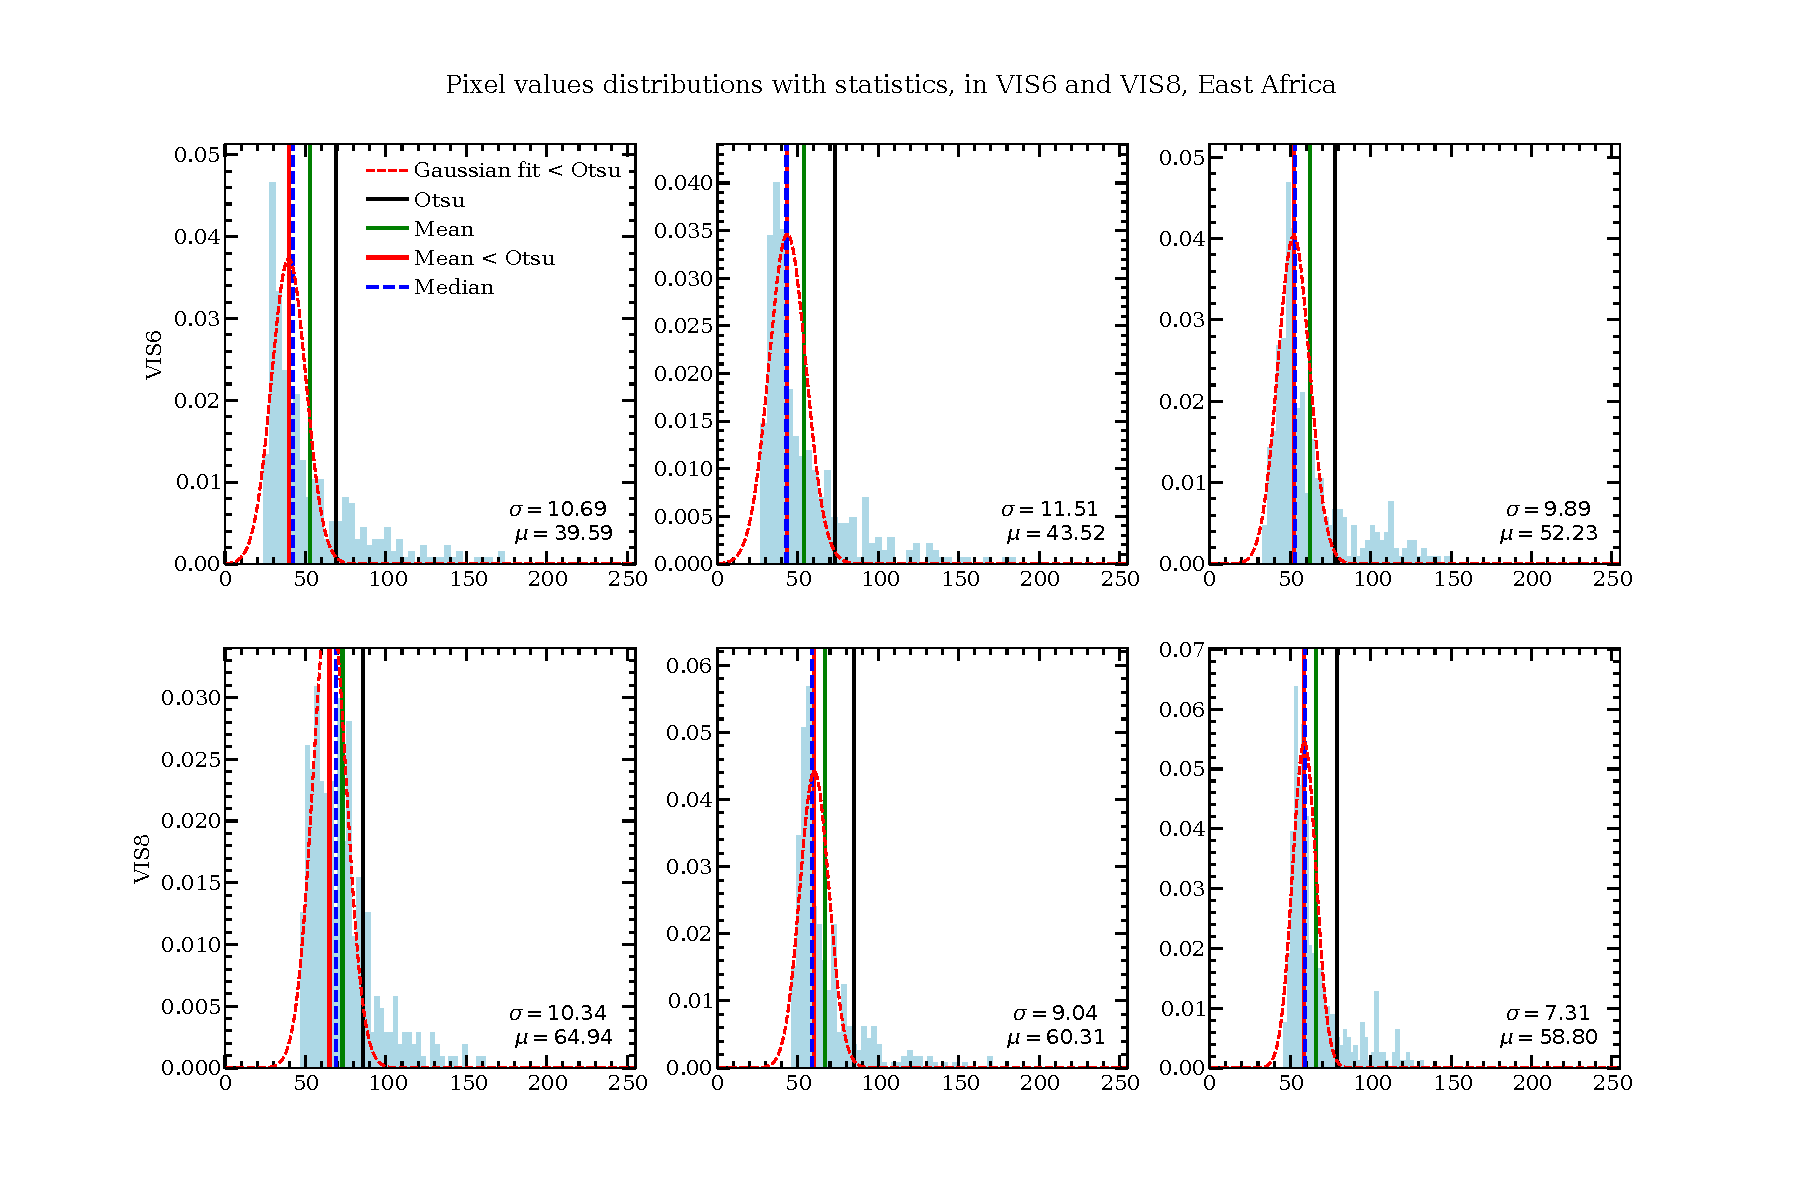
\includegraphics[width=\textwidth]{figures/pixel_distributions_stats_eastafrica}
  \caption{As in Figure \ref{fig:pix_d_south}, but for East Africa.}
  \label{fig:pix_d_east}
\end{figure*}

\subsection{Cloud coverage}
\label{sec:disc:cc}
When calculating monthly values for cloud fraction, we have to average
over all of the days for a given month. In calculating this average we
could use either the mean or the median, and then estimate the
uncertainty based on the standard deviation or interquartile range
(IQR). Figure \ref{fig:cf_dist_south} shows the distribution of cloud
fraction values within a month for South Africa, and Figure
\ref{fig:cf_dist_east} shows the same but for East Africa. The
interesting point here is that the distribution changes from being
skewed to looking almost normally distributed, due to the seasonal
modulation (discussed in depth in Section \ref{sec:disc:rain}). Figure
\ref{fig:cf_dist} shows that using the mean as the average and the
standard deviation as an estimate of uncertainty for July (January) in
South Africa (East Africa) is clearly not appropriate, as they are
skewed by the long tail. For these months the median and IQR do a much
better job of selecting the average and its uncertainty. In January
(July) for South Africa (East Africa) the mean and standard deviation
could be used, but the median is still useful even when the data
appear to be normally distributed and it is much better to use a
statistical measure that is appropriate for all the data, rather than
one that is suited to one part of the dataset but completely off for
the rest.
\begin{figure*}
  \centering
  \begin{subfigure}{0.45\textwidth}
    \centering
    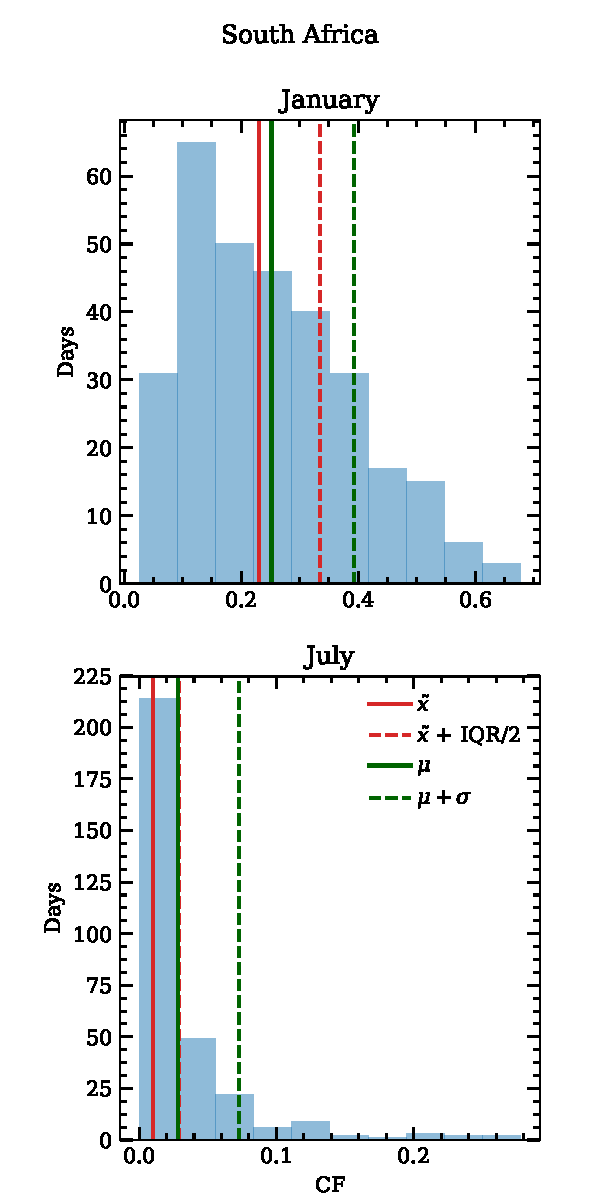
\includegraphics[width=\textwidth]{figures/cf_monthly_dist_capetown}
    \caption{South Africa. Note how in January the cloud fractions
      appear to be normally distributed, while in July they are skewed
      toward lower values. This is due to seasonal modulation, which
      is discussed in depth in Section \ref{sec:disc:rain}.}
    \label{fig:cf_dist_south}
  \end{subfigure}
  ~
  \begin{subfigure}{0.45\textwidth}
    \centering
    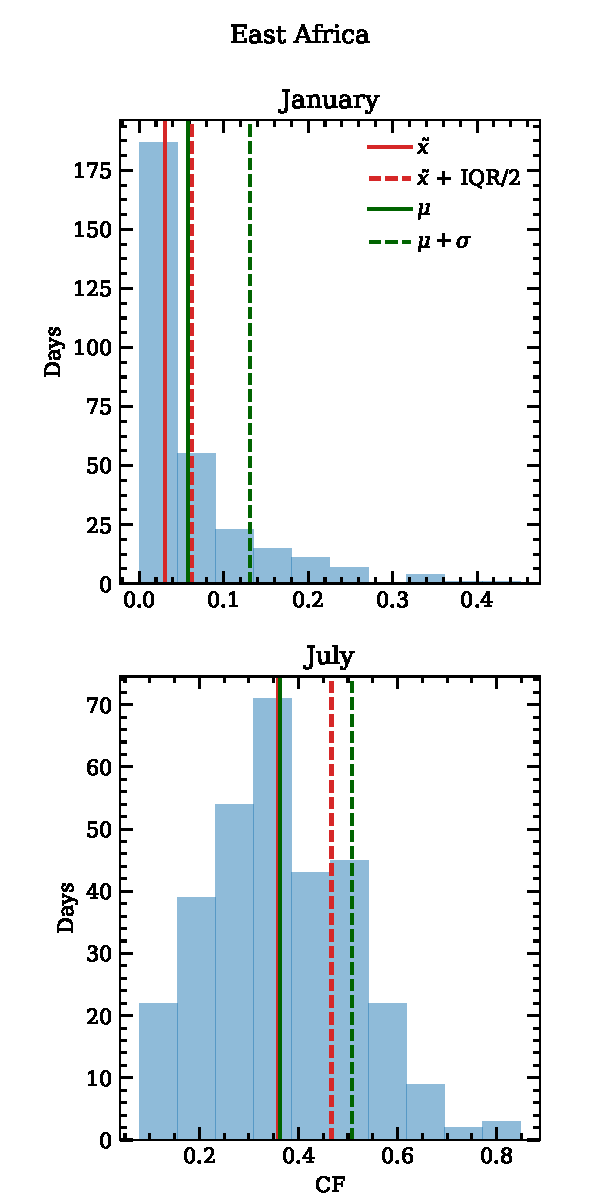
\includegraphics[width=\textwidth]{figures/cf_monthly_dist_eastafrica}
    \caption{East Africa. Note how the distributions are swapped
      compared to Figure \ref{fig:cf_dist_south}. Here the values for
      January are skewed toward lower values, while the values for
      July look more normally distributed.}
    \label{fig:cf_dist_east}
  \end{subfigure}
  \caption{Distribution of cloud fraction values for South Africa and
    East Africa. Top: distribution of all values for January, over the
    years 2008--2017. Bottom: distribution of all values for July, for
    the same year range. Shown in solid red is the median values
    $\tilde{x}$, dashed red the median and half the interquartile
    range (IQR), solid green the mean $\mu$ and dashed green the mean
    and one standard deviation $\sigma$.}
  \label{fig:cf_dist}
\end{figure*}

\subsubsection{Rainfall}
\label{sec:disc:rain}
Here we discuss the relationship between cloud coverage and rainfall,
as shown in Figure \ref{fig:cf_rf}. For South Africa (Figure
\ref{fig:cf_rf_south}) it is clear that cloud coverage follows the
same seasonal modulation as rainfall. The rainy season
(November--March) coincides with winter in the southern hemisphere and
the dry season (April--October) with summer. For East Africa the dry
season (December--January) falls in the northern hemisphere winter,
while the rainy season (March--July) falls mostly in summer. The
overall trend of cloud coverage and rainfall is similar here, but
there is some slight disagreement as to where the peak lies. This
neatly highlights one of the benefits of using cloud coverage
determined via remote sensing as a proxy over rainfall data, for
studying general trends. Precipitation data is inherently
inhomogeneous -- there must be a station located somewhere to detect
the rain. For Figure \ref{fig:cf_rf_east} the rainfall station was
located in Ethiopia, while the cloud coverage data is calculated by
taking a box average over the whole of Ethiopia, and parts of Kenya
and Somalia too. Hence we can get a much better idea of the
\emph{general} rainfall dynamics, compared to the \emph{local}
information garnered from precipitation data \footnote{This does not,
  of course, mean that having local data is not useful in different
  situations, for example in comparing rainfall between different
  types of land.}. East Africa is a complex climatic system but, as
the rainfall variability is spatially coherent and driven by
global-scale dynamics, it is reasonable to study the region on the
large scale \citep{nicholson1996b}.
  
%% A key point to note is that any climate effects will depend on what would usually be happening in that season.

%% An interesting point to note is that South African rainfall varies by over 50mm while East African rainfall varies by around 5mm. Drought?

\subsubsection{SSTA}
\label{sec:disc:ssta}
Here we will discuss how cloud coverage responds to SSTAs, beginning
with South Africa (Figure \ref{fig:cf_t_south}). Between July 2009 --
March 2010 and November 2014 -- May 2016 the ENSO is in its warm phase,
\elnino{}. If there is a response to the positive ONI in 2009/2010,
then Figure \ref{fig:cf_t_south} indicates that it is insignificant in
our data. During the 2014--2016 \elnino{} period we observe negative
cloud fraction anomalies from November 2014 which switch to positive
cloud fraction anomalies around January 2015. In July 2015, the cloud
fraction anomalies peak and turn around again, steadily decreasing
toward a minimum in March 2016, roughly 3 months after the ONI peaked
in December 2015. Important to note is that in the same time period
that the positive cloud fraction anomalies peak, strong positive SWIO
SSTAs ${>}0.5\degc$ are also present. Perhaps here the dearth of cloud
coverage that we expect to see in South Africa due to an \elnino{}
event is countered by enhanced SSTAs in the SWIO before the strong ONI
again triumphs in suppressing cloud coverage.

In our time range there are technically four \nina{} periods: November
2008 -- March 2009, June 2010 -- May 2011, July 2011 -- March 2012 and
August 2016 -- December 2016. Two of the periods are separated by only
a month where the ONI dipped to $-0.4\degc$. Following the peak of the
2008/2009 \nina{} in January 2009, there was a significant spike in
the cloud fraction in March 2009.  This positive anomaly is present
despite negative SWIO SSTAs. Similarly, following the peak of the
2010/2011 \nina{} in October 2011, there is a significant positive
cloud fraction anomaly in December of the same year. The 2011/2012 and
2016 \nina{} events both precede positive cloud fraction anomalies by
two months or so, however, due to the large uncertainty on the values,
it would be misguided to label these as significant. It is also worth
noting that the ONI magnitude for the 2011/2012 and 2016 \nina s are
relatively small in comparison to the other events in our time period.

We move now to East Africa, shown in Figure
\ref{fig:cf_rf_east}. Immediately before and during the growth of the
2009/2010 \elnino{} we observe negative cloud fractions. Around
October 2009 the cloud fraction anomalies climb rapidly before peaking
in January 2010 at the largest value we observe in our entire dataset
(CF$_{\sigma}=0.88\pm0.59$). This peak in cloud anomalies comes a month
after the peak of the \elnino{} event in December 2009 and coincides
with positive WTIO SSTAs (${>}0.25\degc$), present since March 2009
which become large (${>}0.5\degc$) in January 2010. Comparing this
response with that of the 2014--2016 \elnino{}, we find that the
negative anomalies present during the growth of \elnino{} are much
more pronounced. The negative cloud anomalies persist from October
2014 to September 2015 and are accompanied in by a dip in WTIO SSTAs
from December 2014 to February 2015, whereupon the WTIO SSTAs become
positive and remain so until June 2016. The interesting point here is
that the cloud fraction anomalies remain negative for so long despite
both strong ONI and WTIO SSTAs being present. \cite{parhi2016} suggest
a mechanism for this in that tropical eastern Africa is affected most
greatly by the mature phase of \elnino{}, through warming of the
neighbouring Indian Ocean (reflected in the positive WTIO SSTAs
between February 2015 and June 2016). The suppression of cloud
coverage evident in the growth phases of both \elnino{} events could be
due to the coincidence of this phase and the `dry' season of East
Africa (shown in Figure \ref{fig:cf_rf_east}), exacerbating the
already present dearth of precipitation. Whatever the mechanism, it is
an interesting result.

Our data show no significant response to the 2008/2009 \nina{} in East
Africa. For the both the 2010/2011 and 2011/2012 \nina{} events, the
cloud fraction anomalies and WTIO SSTAs appear to closely follow the
ONI, after a lag. Following the \nina event that begins in June 2010,
negative cloud fraction anomalies begin to appear in October 2010
after transitioning from the strong positive anomalies of January
2010. The ONI then dips to $-0.4\degc$ in June 2011 and the cloud
fraction anomalies become positive again. This \nina{} event then has
something of a resurgence, the next month dropping back below
$-0.5\degc$, with the minimum occurring in October/November
2011. Cloud fraction anomalies become negative again in November 2011
and they become quite negative, falling to $-0.4$ in February 2012,
until April 2012 whereupon they revert to being positive. Throughout
this, the WTIO SSTAs are closely tracking the cloud fraction
anomalies. This would appear to indicate that if the \nina{} is
affecting the cloud coverage, it is also affecting the SSTAs. For the
2010/2011 \nina{}, the minimum WTIO SSTAs precedes the cloud fraction
anomaly minimum by one month, while for the 2011/2012 \nina{} they
fall on the same month. This could indicate that \nina{} reduces cloud
coverage in East Africa via lowering SSTs in the WTIO.

From our analysis of cloud coverage for East and South Africa we are
able to draw some tentative conclusions. For South Africa, we would
expect \elnino{} events to precede drought conditions
\cite{TODO}. This partly exhibited by a reduction in cloud coverage
following the mature phase of the 2014--2016 \elnino{}, however we
don't observe a corresponding signal from the 2009/2010
\elnino{}. Following the 2008/2009 and 2010/2011 \nina{} events we
observe the expected (found by \cite{nicholson2000} for rainfall)
increase in cloud overage. It is also clear that SWIO SSTAs play a
crucial role in South African cloud coverage, although their relation
to the ENSO is unclear. \cite{webster1999} use the 1997/1998 \elnino{}
event to suggest that, despite the coincidence of western IO SSTAs and
an, the SSTAs were more likely due to internal dynamics than external
forcing. On the other hand, \cite{alexander2002} propose that there is
a clear link between Pacific and Indian Ocean SST anomalies,
particularly in boreal winter and spring. In East Africa, we observe
that \elnino{} events generally lead to an increase in cloud coverage,
as reported by \cite{TODO}. However we also see that this increase in
cloud coverage is usually only present after the mature phase of the
\elnino{} event, and that the growth phase leads to a suppression of
cloud coverage. \cite{parhi2016} suggest a mechanism for this whereby
\elnino{} conditions lead to a warming of the WTIO, in turn generating
more clouds. Indeed, we do observe that WTIO SSTAs follow East African
cloud fraction anomalies very closely, either preceding the anomalies
by a month or occurring simultaneously. A possible reason for the
suppression of cloud coverage in the growth stages of the \elnino{}
events could be that this phase usually occurs during East Africa's
`dry' season, and so exacerbates the scarcity of cloud already present
\cite{TODO}. The signal for \nina{} events is much more obscure,
although it appears as if negative cloud fraction anomalies occur
during these years, and that these anomalies are also very strongly
correlated with WTIO SSTAs. This indicates the WTIO as a possible
mediator for ENSO effects in East Africa.

\subsection{Vegetation} 

\subsubsection{Spatial response}
Looking first at South Africa (Figure \ref{fig:ndvi_sp_south}) the
NDVI distribution for DJF \elnino{} found in our study are consistent
with those reported in \cite{anyamba2002} for the 1997/1998 \elnino{}
event. Our distribution for DJF \elnino{} is also consistent with the
rainfall anomaly distribution in \cite{deoliveira2018}. Comparing our
distribution for DJF \elnino{} with the distribution for JJA \elnino{}
we find that the negative anomalies intensify, with small regions of
positive anomaly appearing in the north and southern coastal
regions. This effect is not consistent, aside from the appearance of
positive anomalies on the southern coastal region, with the rainfall
anomaly distribution presented in \cite{deoliveira2018}. This may be
due to disparities in the way we have calculated anomalies, or may be
an effect of the seasonal modulation of rainfall and the lag of
vegetation growth. Moving on to the bottom panels of Figure
\ref{fig:ndvi_sp_south}, our distribution for DJF \nina{} shows
positive anomalies concentrated in the east, which is consistent with
the distribution of NDVI anomalies found by \cite{anyamba2002} for the
1999/2000 \nina{} event. \cite{deoliveira2018} report a similar
pattern of rainfall anomalies for DJF. For JJA we find positive
anomalies distributed to the west and negative anomalies along the
southern coast, which is inconsistent with the rainfall anomalies
found by \cite{deoliveira2018}.

\subsubsection{Temporal response}

The East African NDVI signal investigated by \cite{anyamba2002} shows a strong
correlation with their chosen ENSO index (NINO 3.4). The strong \elnino{} in the
period 1997--1998 is followed shortly thereafter with a strong positive NDVI
signal from late 1998 to early 1999. Thereafter follows a reversal from
\elnino{} to \nina{}. Their NDVI trend in this period is less obviously
influenced by NINO 3.4. Though the authors deemed it significant, stating: ``In
general, there was a reversal in NDVI response patterns in East (southern) from
positive (negative) during the \elnino{} in 1997/98 to negative (positive)
during the \nina{} event in 1999/2000.'' We have available, in the time span
covered by our data, two similar events showing a reversal from \elnino{}
conditions to \nina{} conditions. We may then look here, where ENSO effects were
deemed strongest, for comparison with our results.

The period May 2009 -- May 2011 shows the transition from strong \elnino{}
conditions (reaching peak magnitude in late 2009) to strong \nina{} conditions
(reaching peak magnitude in late 2010).

Figure \ref{fig:ndvi_t_south} shows NDVI response in South Africa. During the
above EN/LN reversal period, there is no clear response by NDVI. The more
interesting relationship in this period is between NDVI and SWIO where both seem
to vary in step from January 2010. The strongest positive NDVI anomaly for South
Africa occurs mid 2011 with no clear direct correlation from ONI. For East
Africa, Figure \ref{fig:ndvi_t_east}, there is a more fruitful trend: the 2009
peak positive ONI is followed approximately three months later by a strong
positive NDVI anomaly signal. The following peak negative ONI is matched by a
negative NDVI anomaly. The lag between peak negative ONI and NDVI anomaly is
here less pronounced, possibly reduced by the WTIO which has begun warming in
turn leading to a sooner uptake in NDVI.

The second notable period of January 2014--September 2016 also shows a reversal
from \elnino{} (reaching peak magnitude in late 2015) to \nina{} (reaching peak
magnitude in mid 2016), though the negative ONI here is less pronounced than
that of late 2010.

The NDVI response in South Africa during this period shows a negative anomaly
during the peak positive ONI. NDVI then returns to typical values, on to the end
of the data. The negative response in NDVI to positive ONI here is not
necessarily contrary to the results of \cite{anyamba2002} whose results for
South Africa show a mostly positive NDVI anomaly throughout their results,
apparently unaffected by the strong EN/LN reversal.

Interestingly, Anyamba's NDVI anomaly show more correlation in both East and
South Africa with the WTIO and SWIO and indices respectively. During times of
neutral ONI, we also see this trend, namely during the period January
2012--January 2015. However, when ONI becomes significant (EN or LN conditions
prevalent), NDVI and WTIO/SWIO correlation becomes less prominent in our
results.

\subsection{Limitations}
There are some limitations to our study that we will acknowledge and
discuss here. First and foremost of these is our small sample size;
data were only available to us over the period 2008--2017. As discussed
in Section \ref{sec:analysis}, the climate is an inherently noisy
system (in fact, predicting the weather spawned one of the earliest
studies of chaos by \cite{lorenz1963}) and so lots of data are needed
to observe any trends, usually at least a decade's worth.

A consequence of a small amount of data is that it leads to a small
baseline from which to calculate anomalies. The baseline we use is
derived from our entire dataset which, as can be seen from Figures
\ref{fig:cf_temporal} and \ref{fig:ndvi_temporal}, contains a lot of
ENSO events. For such a small period (8 years), it is unlikely that we
have managed to capture a representative average baseline. This error
will propagate into our anomalies, which are calculated from the
baseline.

A further stumbling block is that our thresholds do not work well with
large deserts. We have addressed this problem by analysing non-arid
regions, although this clearly is not an optimal solution. It would be
better in future work to employ other bands, particularly in the near
infra-red, to distinguish between cloud and desert (see
\cite{derrien1993} for an example). Any error in the thresholds will
impact all products produced using them and, since the thresholds are
essential to the project, it is important to consider and improve on
any sources of error.

%% Local Variables:
%% fill-column: 80
%% TeX-master: "report"
%% End:
